\documentclass[9pt]{beamer}

%-------------------------------------------------
%   THEMES & PACKAGES
%-------------------------------------------------
\usetheme[progressbar=frametitle]{metropolis}
\usepackage{graphicx}
\usepackage[export]{adjustbox}

%-------------------------------------------------
%   COMMON INFO
%-------------------------------------------------
\newcommand{\hmwkTitle}{Bishop Book Section 3.1 -- 3.4}
\newcommand{\hmwkDueDate}{October 27, 2016}
\newcommand{\hmwkClass}{Advanced Mathematics for Robotics and Control}
\newcommand{\hmwkClassShort}{AMRC WS2016}
\newcommand{\hmwkAuthorFullName}{Minh H. Nguyen}
\newcommand{\hmwkAuthorLastName}{Nguyen}
\newcommand{\hmwkAuthorEmail}{minh.nguyen@smail.inf.h-brs.de\\
    bach.ha@smail.inf.h-brs.de}
\newcommand{\hmwkAuthorInstitute}{BRS University of Applied Sciences}


%-------------------------------------------------
%   TITLE
%-------------------------------------------------
\title{\hmwkClass}
\subtitle{\hmwkTitle}
\date{Lecture date: \hmwkDueDate}
\author[\hmwkAuthorLastName]{\hmwkAuthorFullName}
\titlegraphic{\hfill
\includegraphics[height=0.7cm]{../../images/h-brs-logo.jpg}}

\setbeamertemplate{footline}[text line]{%
    \parbox{\linewidth}{\vspace*{-8pt}\hmwkClassShort\hfill\hmwkTitle\hfill\insertshortauthor\hfill\insertpagenumber}}
\setbeamertemplate{navigation symbols}{}

%-------------------------------------------------
%   BEGIN
%-------------------------------------------------
\begin{document}

%-------------------------------------------------
\maketitle

%-------------------------------------------------
%-------------------------------------------------
\begin{frame}{Linear Basis Function Models}
    \begin{alertblock}{Linear model for regression}
        \[ y(\mathbf{x}, \mathbf{w}) = w_0 + \sum_{j=1}^{M-1} w_j \phi_j(\mathbf{x}) \]
        where $\phi(\mathbf{x})$ are \textit{basis functions} and $M$ is the number of parameters. $\phi_0(x) = 1$ can be added to achieve the form $y(\mathbf{x}, \mathbf{w}) = \mathbf{w}^T \phi(\mathbf{x})$
    \end{alertblock}
    \begin{alertblock}{Basis functions}
        \begin{center}
            \setlength{\fboxsep}{0.5pt} %
            \setlength{\fboxrule}{0.5pt}
            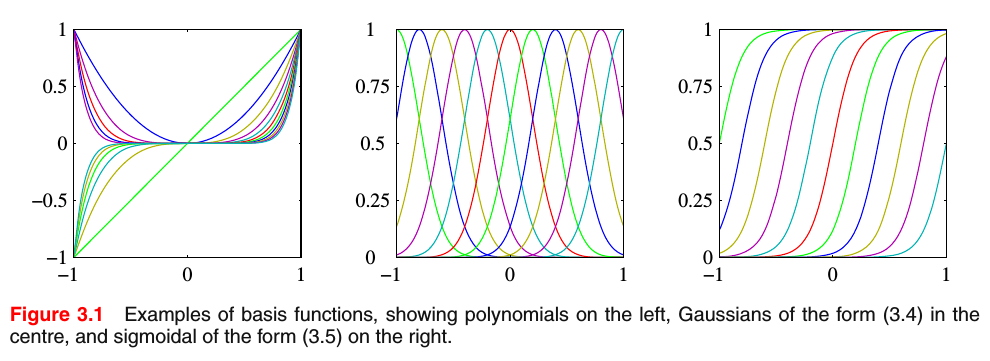
\includegraphics[width=10cm,fbox]{../images/Bishop_MachineLearning_Figure3-1.png} %
        \end{center}
    \end{alertblock}
\end{frame}

%-------------------------------------------------
%-------------------------------------------------
\begin{frame}{Linear Basis Function Models}
    \begin{alertblock}{Maximum likelihood and least squares}
        With target variable $t = y(\mathbf{x}, \mathbf{w}) + \epsilon$, where $\epsilon$ is a zero mean Gaussian noise with precision $\beta$ and $y(\mathbf{x}, \mathbf{w})$ is some deterministic function:
        \[ p(t | \mathbf{x}, \mathbf{w}, \beta) = \mathcal{N}\left( t | y(\mathbf{x}, \mathbf{w}), \beta^{-1} \right) \]
        Given data set of inputs $\mathbf{X} = \{x_1,...,x_N\}$ with targets $t_1,...t_N$, likelihood function:
        \[ p(\mathbf{t} | \mathbf{X}, \mathbf{w}, \beta) = \prod_{n=1}^{N}\mathcal{N}(t_n | \mathbf{w}^T \phi(\mathbf{x}_n), \beta^{-1}) \]
    \end{alertblock}
\end{frame}

%-------------------------------------------------
%   END
%-------------------------------------------------
\end{document}
